\subsection{Gliederung}
\includepdf[pages=3-4]{./Hausaufgaben/9_Projektskizze_BA/main.pdf}
% 0 Abstract\\
% 1 Einleitung\\
%   1.1 Motivation\\
%   1.2 Zielstellung\\
%   1.3 Aufbau der Arbeit\\
% 2 Theorie\\
%   2.1 Arbeitsplatzgestaltung\\
%     2.1.1 Gestaltungsrichtlinien\\
%     2.1.2 Telepräsenz\\
%       Immersion\\
%       Intuition\\
%     2.1.3 Anthropometrie\\
%       menschlicher Sehraum\\
%       Oberkörperproportionen\\
%   2.2 visuelle Kommunikation\\
%     2.2.1 Aufnahme - Fish-Eye Kamera\\
%     2.2.2 Vorverarbeitung - radiale Verzerrung\\
%     2.2.3 Darstellung - Head Mounted Display\\
%   2.3 Robotik\\
%     2.3.1 Roboterarten\\
%     2.3.2 Manipulatorsteuerung\\
%     2.3.3 anthropomorphe Roboterkinematik\\
%     2.3.4 Server/Datenübertragung\\
%     2.3.5 Stand der Technik/bisherige Lösungsansätze\\
%   2.4 Forschungsfrage\\
% 3 Methoden\\
%   3.1 Motion Tracking\\
%   3.2 Manipulator des Instituts\\
%   3.3 Bildübertragung\\
%     3.3.1 HTC Vive\\
%     3.3.2 SteamVR\\
%     3.3.3 StereoStitch Live\\
%     3.3.4 Kodak Pixpro SP360 4K\\
%   3.4 Robot Operating System\\
% 4 Konzept\\
% 5 Umsetzung\\
%   5.1 Kontrolle des Roboterarms\\
%     5.1.1 udplistener.py\\
%     5.1.2 Angles.msg\\
%     5.1.3 roscore, rosserial\_arduino\\
%     5.1.4 Arduino\\
%   5.2 Bildübetragung\\
%   5.3 Hardwaresetup\\
%     5.3.1 Kameraposition\\
% 6 Funktionsvalidierung\\
% 7 Diskussion und Ausblick\\
% 8 Literaturverzeichnis
